\documentclass[a4paper, 12pt, notitlepage]{report}

\usepackage[utf8]{inputenc} % set input encoding (not needed with XeLaTeX)
\usepackage[english]{babel}
\usepackage{amsmath}
\usepackage{amsfonts} % if you want blackboard bold symbols e.g. for real numbers
\usepackage{amssymb}
\usepackage{stmaryrd}
\usepackage{multicol}
\usepackage{tikz}
\usepackage{tkz-tab}
\usepackage{enumitem}
\setcounter{secnumdepth}{5}
\usepackage{mathtools}
\usepackage{setspace}

\setlength{\parskip}{1em}

\graphicspath{{images/}}

\usepackage{color} % For source code appendix
\definecolor{green2}{rgb}{0,0.6,0}
\definecolor{gray2}{rgb}{0.5,0.5,0.5}
\definecolor{mauve2}{rgb}{0.58,0,0.82}

\usepackage{hhline}

\usepackage{listings} % To insert code
\lstset{
    basicstyle=\footnotesize,
    breaklines=true,
    commentstyle = \color{green2},
    keywordstyle=\color{blue},
    numbers = left,
    numbersep = 5pt,
    numberstyle = \tiny\color{gray2},
    stringstyle = \color{mauve2},
    tabsize=2,
    language = Java
}

\usepackage{xcolor}
\usepackage{hyperref}
\hypersetup{
    colorlinks=true,
    linkcolor=blue,
    filecolor=blue,
    urlcolor=blue,
}

\usepackage{graphicx} % if you want to include jpeg or pdf pictures

\title{Inversion of Control Programming Assignment} % change this
\author{Kevin León Sandoval, B53845\\Josué León Sarkis, B53846\\Elías Calderón Calderón, B51322} % change this
\usepackage{datetime}
\newdate{date}{01}{10}{2017}
\date{\displaydate{date}}

\bibliographystyle{plain}

\begin{document}

%%%%%%%%%% PRELIMINARY MATERIAL %%%%%%%%%%
\maketitle
\begin{center}
Escuela de Ciencias de la Computación e Informática
\\[12pt]
Universidad de Costa Rica. % change this
\end{center}
\thispagestyle{empty}

\newpage

\tableofcontents 


%%%%%%%%%% MAIN TEXT STARTS HERE %%%%%%%%%%

%%%%%%%%%%%%%%% INTRODUCCIÓN %%%%%%%%%%%%%%
\chapter{Introduction}
%
\section{Summary}
%
\textit{Software engineering} is a Computer Science branch, based on the two concepts software and engineering, and consisting on a set of methods, models, tools, and techniques that facilitate software development. 

One of the main goals of software engineers is to reduce this process complexity, which is naturally very high. Software engineering has a lot of design patterns and programming models, that can be used when creating software systems. One of the most used and famous design patterns is \textit{Dependency Injection}. Dependency injection removes the dependencies between objects from their internal composition, and handles them by itself in order to separate the programs in more parts, making a program's objects work independently from others. 

In the other hand, we have Inversion of control, this technique consists in, redundantly, inverting the flow of the program execution. This means, that the developer no longer holds the main control of the program, and it is now driven by a framework. Merging this with Dependency injection, gives us a framework that is in charge of creating and controlling the dependencies of each object and injecting them, only when needed, increasing the modularity. 

An Inversion of Control container is a very complex program that requires a variety of elaborated algorithms and patterns to successfully perform its job. The term was popularized in 1999 by the computer scientist Stefano Mazzochi and since then, different frameworks based on this principle have been developed.

This document presents the documentation of the implementation of NAIoCC(\textit{Not Another Inversion of Control Container}). The documentation includes the flow diagram, the class diagram, the description of the solution, and the metadata configuration for both XML and Java annotations.


%%%%%%%%%%%%%%%% SIMULACIÓN %%%%%%%%%%%%%%%
\chapter{Inversion of Control Container}
%
\section{System description}
%
The inversion of control supports the following functionalities:
\begin{itemize}
    \item[$1.$] Dependency injection:
    \begin{itemize}
        \item[$a)$] Setters.
        \item[$b)$] Constructor.
    \end{itemize}
    \item[$2.$] Scope:
    \begin{itemize}
        \item[$a)$] Singleton.
        \item[$b)$] Prototype.
    \end{itemize}
    \item[$3.$] Lifecycle:
    \begin{itemize}
        \item[$a)$] Initialization.
        \item[$b)$] Destroy.
    \end{itemize}
    \item[$4.$] Autowiring:
    \begin{itemize}
        \item[$a)$] By Name.
        \item[$b)$] By Type.
        \item[$b)$] Constructor.
    \end{itemize}
    \item[$5.$] Configuration Format:
    \begin{itemize}
        \item[$a)$] XML.
        \item[$b)$] Annotations.
    \end{itemize}
    \item[$6.$] Extra features:
    \begin{itemize}
        \item[$a)$] Lazy Loading.
        \item[$b)$] Stereotype annotations.
    \end{itemize}
\end{itemize}

\section{XML Configuration}

To use the container, the user has to define the beans and the information to create them(\textit{metadata}) in an XML file. The XML file is read by creating an \textit{XML Bean Factory}.

The following concepts are the ones that NAIoCC supports for its XML configuration:

\begin{itemize}
    \item \textbf{Bean} is an abstract object, for the dependency injection, that is created by the bean factory and it is saved in the inversion of control container. It has \textbf{id, class, scope, init, destroy, lazy-generation and autowire}. 
    \item \textbf{Id} is the unique identification for each bean. It is obligatory. Its value can not be repeated in different beans.
    \item \textbf{Class} specifies the bean's class path. It is obligatory.
    \item \textbf{Scope} specifies the scope of the bean. It is not obligatory. Its value can be \textbf{Singleton}, which is the default value, or \textbf{Prototype}. Singleton means that just one bean is instantiated and all the requests for that bean use the same instance. \textbf{Prototype} consists in creating a new instance of the bean each time it is requested.
    \item \textbf{Init} consists in the initialization method for a bean. It is not obligatory. This method is called when the bean is instantiated, \textbf{after} injecting all the dependencies of that bean. In the XML file an init default method for every bean can be defined, if a bean specifies a different init method, the default one is overwritten.
    \item \textbf{Destroy} consists in the destruction method for a bean. It is not obligatory. This method is called when the bean is destroyed. In the XML file a destroy default method for every bean can be defined, if a bean specifies a different destroy method, the default one is overwritten. 
    \item \textbf{Lazy-generation} determines if the bean is instantiated when the container is created or when the bean is requested by a user, its effect is only visible in Singletons. It is not obligatory, by default it is set to false. Its value can be the same for different beans. If the value is \textbf{true} the bean is instantiated until it is requested, otherwise \textbf{false}, the bean is instantiated when the container is created. For Prototype scopes, it has no effect since beans are instantiated when requested.
    \item \textbf{Autowire} specifies the automatic way of wiring the dependencies for all the properties found in a bean's class. It is not obligatory, by default it is set to ``none". Its value can be repeated in different beans. The value can be set to ``byName", ``byType", ``constructor" or ``none". It has no effect in a specific attribute or constructor, if the respective \textbf{attribute} or \textbf{constructor} tag is specified.
    \item \textbf{Atomic-autowire} specifies the automatic way of wiring the dependencies for a property in a bean. It is not obligatory, by default it is set to ``none". Its value can be repeated in different beans. The value can be set to "byName", "byType", or "none".
    \item \textbf{Attribute} specifies a bean's attribute, so that it is injected through "setter" methods. It is not obligatory. There can be multiple attributes defined in a bean. It has a \textbf{name}, and either a \textbf{ref} or a \textbf{value} (for primitive types), but not both.
    \item \textbf{Name} identifies the name of the attribute to inject. It is obligatory. Its value can not be repeated inside the same bean.
    \item \textbf{Constructor} is used to define constructor injection and specify its parameters. It is not obligatory. It is unique for a bean, therefore there can only be one Constructor tag inside a bean's configuration.
    \item \textbf{Param} identifies a constructor's argument. It is obligatory. It can have \textbf{type}, \textbf{index} or both. It can also have \textbf{value} or \textbf{ref}, but not both.
    \item \textbf{Type} identifies the type for a  constructor's argument. It is not obligatory.
    \item \textbf{Index} identifies the index in the argument's array for a constructor's argument. It is not obligatory, and its value must be unique inside a bean's constructor.
    \item \textbf{Value} identifies the attribute's value or argument's value. It is not obligatory. Its value is not unique.
    \item \textbf{Ref} makes reference to a declared bean ID for any other bean in the XML. It is not obligatory. The reference is unique but can be used by multiple beans.
    \item \textbf{Annotations Classes} Indicates that there are annotations in some classes. There can be just one annotationsClasses tag in the XML configuration.
    \item \textbf{Class} tag determines a class which contains annotations. It has an attribute called \textbf{path}, which specifies the path of the respective class.
    \item \textbf{Path} has the name of the class with annotations. It can be just one per \textbf{class} tag.
\end{itemize}
\newpage
XML structure:
\begin{lstlisting}[numbers = none,]
<xml version = "1.0" encoding = "UTF-8"?>
<beans init="defaultInitMethod" destroy="defaultDestroyMethod">
    <bean   id = "beanId" class = "package.path.class" 
            scope="Singleton/Prototype" 
            init="methodName" destroy="methodName" 
            lazy-generation="true/false" 
            autowire="byName/byType/none">

            <constructor>
                <param  type="package.path.class" 
                        index="numberIndex" 
                        value="valor"/ref="beanId" />
                        
                <param  ref="beanId" atomic-autowire="byName/byType"/>
                
                <param  type="package.path.class" atomic-autowire="byName/byType"/>                        
            </constructor>

            <attribute  name="nombreAtr" value="valor"/ref="beanId" atomic-autowire="byName/byType"/>
            
            <attribute  name="nombreAtr" atomic-autowire="byName/byType"/>          

    </bean>
    
    <annotationsClasses> 
    
        <class path="package.path.class" /> 
    
    </annotationsClasses>
    
</beans>
\end{lstlisting}

\newpage
\section{Annotations Configuration}

The annotations configuration can be used alongside XML configuration or making an \textit{Annotations Bean Factory}. The following are the annotations concepts and structure:

\begin{itemize}
    \item \textbf{@Bean:} It indicates to the container that the class with the \textbf{@Bean} annotation must be registered as a bean in the container. The bean ID is obligatory, it can be the same name of the class. There can just be one @Bean in a class. It goes above the class definition.
    
    \textit{Structure:}
    \begin{lstlisting}[numbers = none, language = Java]
    @Bean
    public class BeanClass {
        ...
    }
    \end{lstlisting}
    
    \item \textbf{@Scope:} It indicates the bean's scope. There can only be one @Scope in a class. Its values are \textbf{Singleton}, by default, or \textbf{Prototype}.
    
    \textit{Structure:}
    \begin{lstlisting}[numbers = none, language = Java]
    @Bean
    @Scope("Singleton")/@Scope("Prototype")
    public class BeanClass {
    	...
    }

    \end{lstlisting}
    
    \item \textbf{@Init:} It is the initialization method. There can be just one @Init in a class. It determines which method to call when the bean is instantiated.
    
    \textit{Structure:}
    \begin{lstlisting}[numbers = none, language = Java]
    @Bean
    public class BeanClass {
        @Init
        public void initMethod() {
            ...
        }
    }

    \end{lstlisting}
    \item \textbf{@Destroy:} It is the destruction method. There can be just one @Destroy in a class. It determines which method to call when the bean is destroyed. 
    
    \textit{Structure:}
    \begin{lstlisting}[numbers = none, language = Java]
    @Bean
    public class BeanClass {
        @Destroy
        public void destroyMethod() {
        }
    }
    \end{lstlisting}  
    
    \item \textbf{@Lazy:} It determines if the bean is instantiated when the container is created or when the bean is requested by a user, in the case that its scope is Singleton. It is not obligatory, by default it is set to false. If @Lazy is present, the bean is instantiated until it is requested, otherwise the bean is instantiated when the container is created. For Prototype scopes, it behaves the same way as normal since beans are instantiated when requested. There can be just one @Lazy in a class.
    
    \textit{Structure:}
    \begin{lstlisting}[numbers = none, language = Java]
    @Bean
    @Lazy
    public class BeanClass {
        ...
    }
    \end{lstlisting}
    
    \item \textbf{@ClassAutowire:} It specifies to wire the bean's dependencies automatically, "byName", "byType", "constructor" or "none". The default value is "byName". It can be above the class definition, or above a constructor. 
    
    \textit{Structure:}
    \begin{lstlisting}[numbers = none, language = Java]
    @Bean
    @Autowire()
    public class BeanClass {
        ...
    }
    \end{lstlisting}
    
    \item \textbf{@Attribute:} It goes above of the attribute, which is going to be a property of the bean and should have an associated setter method. This annotation has an obligatory parameter, to specify the \textbf{value} or \textbf{ref}(reference) of the attribute. For non-primitive types, it is equivalent to the @Autowired followed by @Qualifier("reference") in the Spring container. There can be multiple @Attribute in a class.
    
    \textit{Structure:}
    \begin{lstlisting}[numbers = none, language = Java]
    @Bean
    public class BeanClass {
	
	    @Attribute("2")/@Attribute("ref")
        private int classInt;

        public void setClassInt() {
            ...
        }
    }

    \end{lstlisting}
    
        \item \textbf{@AtomicAutowire:} It goes above of an  attribute or the constructor. It states that the property must be autowired and can be "byName" or "byType". If the type is not indicated, "byType" is assumed firstly and if it doesn't matches with the parameters, "byName" is tried. 
    
    \textit{Structure:}
    \begin{lstlisting}[numbers = none, language = Java]
    @Bean
    public class BeanClass {
	
	    @AtomicAutowire()/@AtomicAutowire("byName"/"byType")
        private int classInt;

        @AtomicAutowire()/@AtomicAutowire("byName"/"byType")
        public BeanClass(){}
        public void setClassInt() {
            ...
        }
    }

    \end{lstlisting}
    
    \item \textbf{@Constructor:} It goes above the constructor that will be used in the bean dependency injection. There can be just one @Constructor in the class.
    
    \textit{Structure:}
    \begin{lstlisting}[numbers = none, language = Java]
    @Bean
    public class BeanClass{
	    @Constructor
	    public BeanClass(. . .){
	    	. . . 
        }
    }

    \end{lstlisting}
    \item \textbf{@Parameter:} It should be present after @Constructor. It indicates the value of one of the parameters of the bean's constructor definition. This annotation has an obligatory parameter, to specify the \textbf{value} or \textbf{ref}(reference).
    
    \textit{Structure:}
    \begin{lstlisting}[numbers = none, language = Java]
    @Bean
    public class BeanClass{
	    @Constructor
	    @Parameter("val1")/@Parameter("ref")
	    public BeanClass(. . .){
	    	. . . 
        }
    }
    \end{lstlisting}
\end{itemize}



%%%%%%%%%%%%%% IMPLEMENTACIÓN %%%%%%%%%%%%%
\chapter{Implementation}
%
\section{Solution description}

In order to achieve a successful implementation of the Inversion of Control container, NAIoCC's team researched about Java Reflection. Java Reflection is a library of Java, which provides the utilities to get important properties of a class, such as the name, fields, methods, constructors, constructor parameters, annotations and other important components. The team also researched about Spring, in the Spring Documentation, to learn how Spring manages the different configurations and flows to get a general idea of how their IoC work and use it for our implementation. 

The team had several meetings, after the research process, to discuss the application domain and define the problem and what was needed. Then we made the design of the implementation, which consisted on a flow diagram and the class diagram. After the design process, we decided how to parse the XML and agreed on using DOM(\textit{Document Object Model}) Parser to read and process the XML configuration file, because it is a very useful and simple tool to do it. DOM Parser processes the main tag as a root of a tree structure, the tags inside as his children, and the properties of the tags as attributes of his children or himself. 

In this way, the general solution from a high level perspective consists on reading the beans' configuration, either from the XML file or Java Annotations classes, via the XMLBeanReader or AnnotationsBeanReader, both of them classes that inherit from the abstract class BeanReader. While reading the configurations, the metadata of each bean is passed to the BeanCreator class, which is in charge of creating each bean with its corresponding basic configuration values and properties. Once the reader finishes reading the properties of a bean, it communicates it to the BeanCreator, for it to pass it to the BeanFactory so that it is added to the container. It is important to highlight that at this point, the beans in the container only hold the metadata, no beans have been instantiated nor autowired.

Once the reader finished reading all the configuration, and with all the beans in the container, the BeanFactory proceeds to check the beans dependencies to detect any cycles and if no cycles were detected, it then instantiates all beans, by iterating through all of them in the beans HashMap and checking important conditions such as their scope, to determine if they should be instantiated now, in the case that it is Singleton and without Lazy Generation, or later when the user requests the bean. 

Moreover, in general terms, when a bean is instantiated, a new instance is created and added to the list of instances in the Bean class, which holds the metadata. When creating the new instance, the dependencies are first autowired and then it is created with the specified constructor or the default one if it wasn't specified. Once the new instance is created, its dependencies are then injected, via the setter methods, if indicated as such.

The process of autowiring can be executed in different ways, depending on the configuration. In the case that it is set to "byName", it searches for a bean in the container, that has the same id as the name specified, in order to wire it. In the case that it is set to "byType", a bean with the respective type of the property is searched in the container, and if it finds it, it autowires it. Finally, if set to "constructor", it is similar to "byName" since it finds the beans with the same name of the parameter in the container, to wire it. 

The injection of dependencies after the bean is instantiated, consists in calling the setter methods of the attributes specified to inject. It does this by finding the setter method for the attribute, using its name and then invoking the method. However, in the case that the bean's configuration belongs to Java Annotations, the object to inject is searched in the container by its name, specified with the @Qualifier annotation, to inject it afterwards. 

It is important to stand out that many exceptions are controlled, in the various scenarios. For example, if the autowire is set to "byType" and no reference is specified, if it finds more than one bean with that type, an exception is throwed. Other exceptions include checking that no two beans can have the same id, references that differ on type with the property, unexisting necessary methods to invoke, etc. 

Finally, the user can also call the shutDownHook method of the BeanFactory, which will iterate through all the beans in the HashMap and destroy all the instances for each bean. 


\newpage
\section{Flow Diagram}

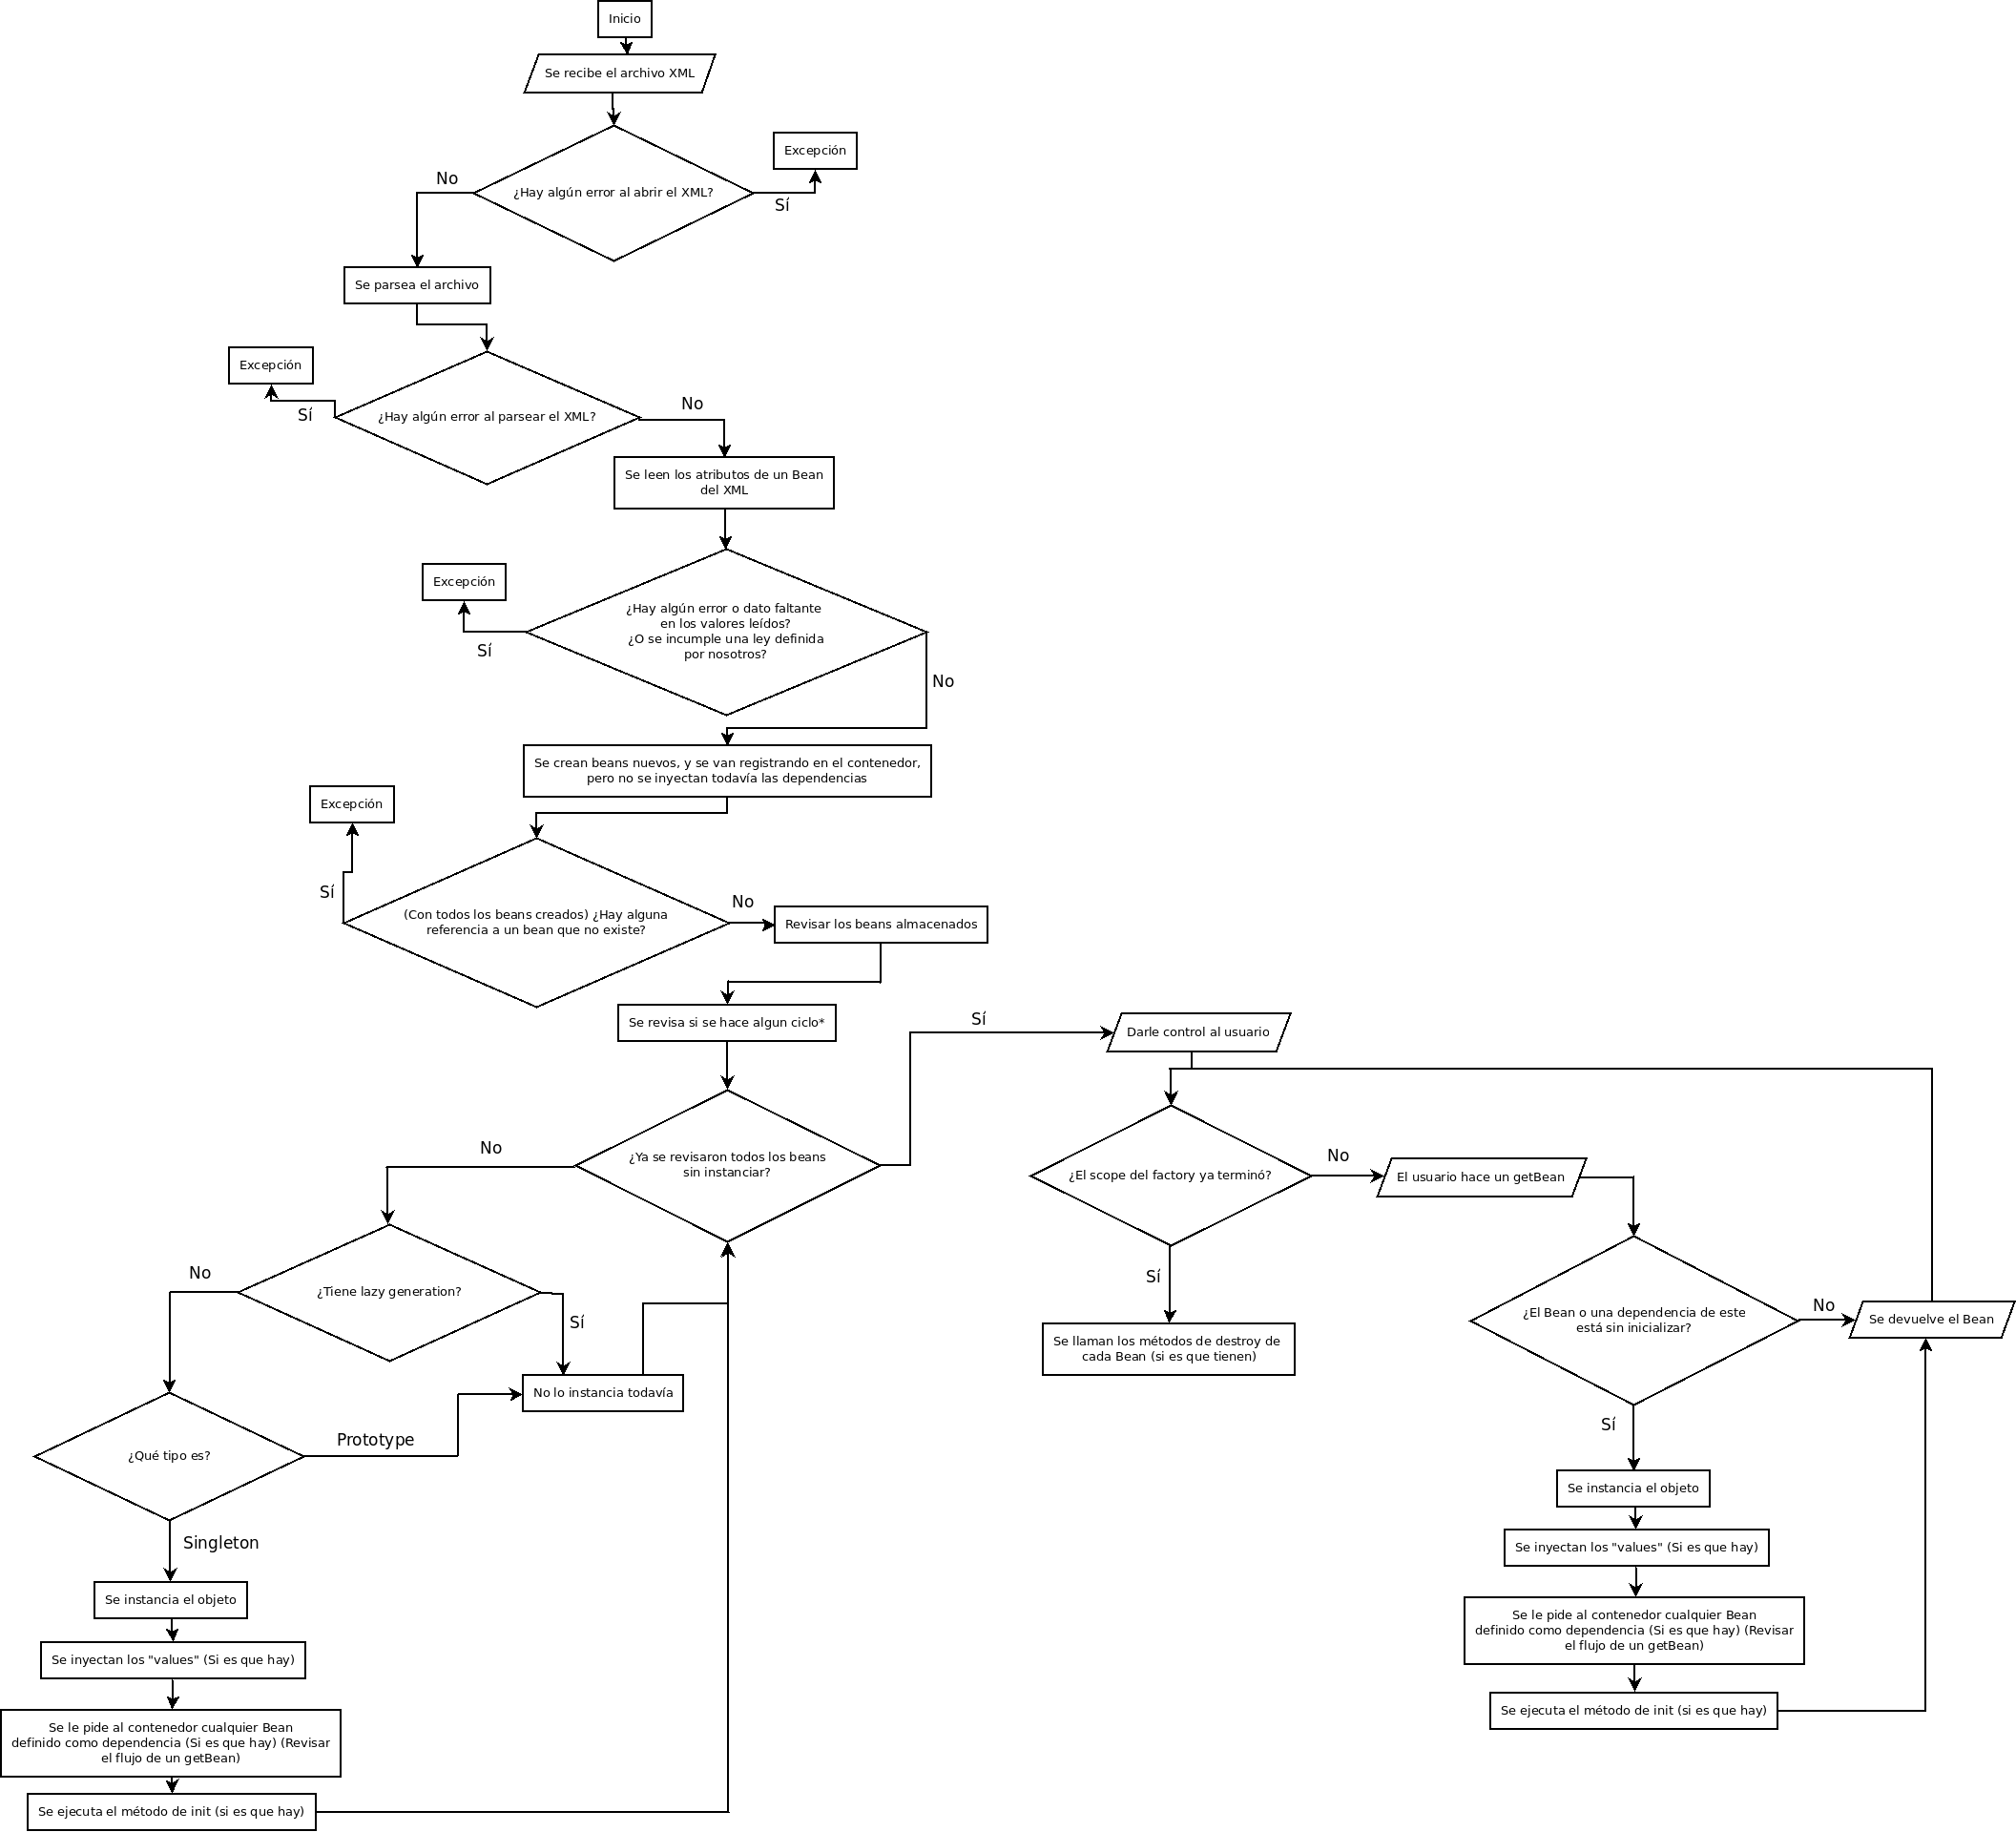
\includegraphics[scale=0.20]{images/flujos.png}

\section{Class diagram}
%
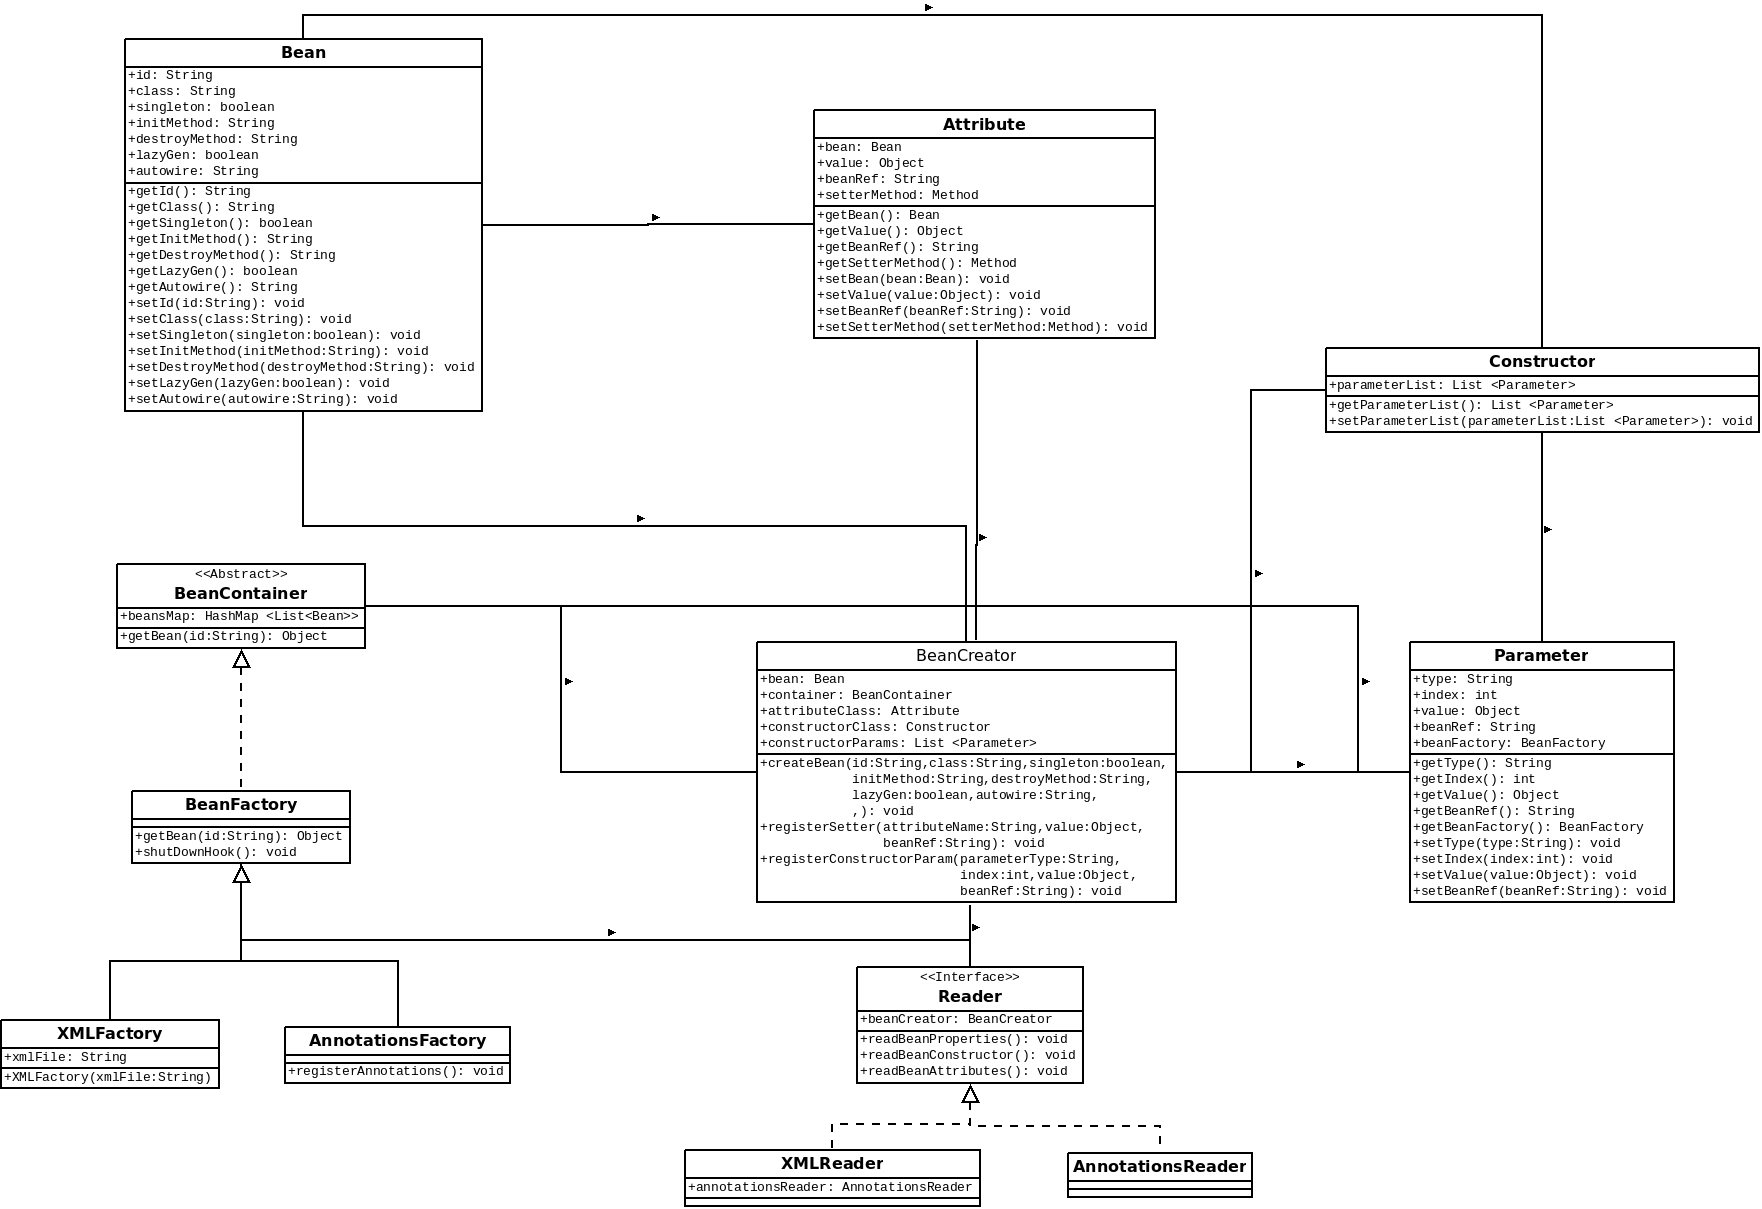
\includegraphics[scale=0.25]{images/ioc.png}

\newpage
%



%%%%%%%%%% APPENDIX %%%%%%%%%%
\appendix
\chapter{Source Code}


\lstinputlisting[title=BeanReader]{src/Reader/BeanReader.java}
\lstinputlisting[title=AnnotationsBeanReader]{src/Reader/AnnotationsBeanReader.java}
\lstinputlisting[title=XmlBeanReader]{src/Reader/XmlBeanReader.java}

\lstinputlisting[title=AtomicAutowire]{src/Annotations/AtomicAutowire.java}
\lstinputlisting[title=Attribute]{src/Annotations/Attribute.java}
\lstinputlisting[title=Bean]{src/Annotations/Bean.java}
\lstinputlisting[title=ClassAutowire]{src/Annotations/ClassAutowire.java}
\lstinputlisting[title=Constructor]{src/Annotations/Constructor.java}
\lstinputlisting[title=Controller]{src/Annotations/Controller.java}
\lstinputlisting[title=Destroy]{src/Annotations/Destroy.java}
\lstinputlisting[title=Init]{src/Annotations/Init.java}
\lstinputlisting[title=Lazy]{src/Annotations/Lazy.java}
\lstinputlisting[title=Parameter]{src/Annotations/Parameter.java}
\lstinputlisting[title=Scope]{src/Annotations/Scope.java}
\lstinputlisting[title=Service]{src/Annotations/Service.java}

\lstinputlisting[title=AnnotationsFactory]{src/Factory/AnnotationsFactory.java}
\lstinputlisting[title=BeanConstructorModule]{src/Factory/BeanConstructorModule.java}
\lstinputlisting[title=BeanCreator]{src/Factory/BeanCreator.java}
\lstinputlisting[title=BeanFactory]{src/Factory/BeanFactory.java}
\lstinputlisting[title=XMLFactory]{src/Factory/XMLFactory.java}

\lstinputlisting[title=AutowireEnum]{src/Bean/AutowireEnum.java}
\lstinputlisting[title=Bean]{src/Bean/Bean.java}
\lstinputlisting[title=BeanAttribute]{src/Bean/BeanAttribute.java}
\lstinputlisting[title=BeanAutowireModule]{src/Bean/BeanAutowireModule.java}
\lstinputlisting[title=BeanConstructor]{src/Bean/BeanConstructor.java}
\lstinputlisting[title=BeanParameter]{src/Bean/BeanParameter.java}
\lstinputlisting[title=BeanProperty]{src/Bean/BeanProperty.java}
\lstinputlisting[title=Scope]{src/Bean/Scope.java}
\lstinputlisting[title=Stereotype]{src/Bean/Stereotype.java}

\lstinputlisting[title=AnnotationsBeanReaderException]{src/Exception/AnnotationsBeanReaderException.java}
\lstinputlisting[title=BeanAtomicAutowireException]{src/Exception/BeanAtomicAutowireException.java}
\lstinputlisting[title=BeanAutowireException]{src/Exception/BeanAutowireException.java}
\lstinputlisting[title=BeanConstructorConflictException]{src/Exception/BeanConstructorConflictException.java}
\lstinputlisting[title=BeanConstructorNotFoundException]{src/Exception/BeanConstructorNotFoundException.java}
\lstinputlisting[title=BeanPropertyException]{src/Exception/BeanPropertyException.java}
\lstinputlisting[title=BeanTypeConflictException]{src/Exception/BeanTypeConflictException.java}
\lstinputlisting[title=IdNotFoundException]{src/Exception/IdNotFoundException.java}
\lstinputlisting[title=InvalidPropertyException]{src/Exception/InvalidPropertyException.java}
\lstinputlisting[title=RepeatedIdException]{src/Exception/RepeatedIdException.java}
\lstinputlisting[title=SetterMethodNotFoundException]{src/Exception/SetterMethodNotFoundException.java}
\lstinputlisting[title=XmlBeanReaderException]{src/Exception/XmlBeanReaderException.java}



%%%%%%%%%% BIBLIOGRAPHY %%%%%%%%%%
\bibliographystyle{unsrt}
\addcontentsline{toc}{chapter}{Bibliography}
\nocite{*}
\bibliography{references}
\end{document}